\chapter{Proposed System}

\section{Problem Statement and Passive Threat Model}
The objective of COBRA-WATCH is to compute a per-alert reliability score $T_{\mathrm{final}} \in [0, 100]$ and actionable tier (\texttt{high\_trust} $\ge 80$, \texttt{medium\_trust} $50\text{--}79$, \texttt{low\_trust} $< 50$) for surveillance alerts without violating legal privacy boundaries or sending intrusive traffic to third-party endpoints.

The system considers four concrete adversarial classes within an explicit passive boundary:
\begin{itemize}
  \item \textbf{Decoy Swapping or MITM Relay ($\mathcal{A}_1$):} An adversary substitutes a camera endpoint behind a reverse proxy or inserts a transcoding relay that lowers resolution or changes banner fingerprints while keeping a clean IP/CVE profile.
  \item \textbf{Stream Freeze or Replay Loop ($\mathcal{A}_2$):} An attacker stalls frame updates, injects pre-recorded looping video segments with realistic natural motion, degrades focus sharpness gradually, covers the lens partially/completely, or shifts camera orientation.
  \item \textbf{Collusive Corroboration ($\mathcal{A}_3$):} Compromised neighbouring devices fabricate rapid cross-camera event confirmations to inflate spatial trust bonuses.
  \item \textbf{API Metadata Spoofing ($\mathcal{A}_4$):} Tampered detection-event payloads attempt to overwrite stored vulnerability posture, replay old nonces, or flood the ingestion endpoint.
\end{itemize}

\textbf{Passive Measurement Constraint:} COBRA-WATCH never opens outbound sockets or TCP probes to external target cameras (legacy active heartbeat modules were permanently deleted from the codebase). OSINT intake uses aggregate search telemetry strictly without exporting target IP lists, and the video analysis subsystem rejects any non-whitelisted remote RTSP stream URI via \texttt{\_assert\_source\_is\_authorized()}.

\section{Proposed Methodology and Techniques}

\subsection{Channel A: Vulnerability Posture ($T_{\mathrm{cve}}$)}
For every indexed camera $d$, Channel~A computes a cyber-posture score $T_{\mathrm{cve}} \in [0, 100]$ strictly from server-side database attributes rather than client-supplied payload assertions:
\begin{equation}
  T_{\mathrm{cve}} = \mathrm{clip}_{[0, U]}\!\Big(100 - 30\,\mathbf{1}[\neg \mathrm{auth}] - \Delta_{\mathrm{cat}} - 20\,\mathbf{1}[\text{owner unknown}] - 15\,\mathbf{1}[\mathrm{stale}] - 10\,\mathbf{1}[\mathrm{lat} > 500] + \beta(k)\Big),
\end{equation}
where $U = 49$ if the camera allows unauthenticated stream access (otherwise $100$), $\Delta_{\mathrm{cat}} \in \{0, 15, 25, 30\}$ reflects CWE vulnerability classes mapped from NVD/CISA KEV/EPSS feeds~\cite{nvd,cisakev,jacobs2021epss}, and $\beta(k) \in \{-10, 0, +20\}$ captures spatial corroboration from $k$ nearby cameras ($k = 0, 1, \ge 2$) protected by velocity limits against collusion~\cite{kipf2017gcn}.

\subsection{Channel B, Tier 1: Passive Banner Drift}
Tier~1 derives a banner fingerprint $\mathcal{B}_d(t) = \langle \mathrm{firmware}, \mathrm{server}, \mathrm{ports}, \mathrm{resolution}, \mathrm{product}, \mathrm{codec}\rangle$ from passive metadata snapshots and computes weighted field divergence:
\begin{equation}
  \mathrm{Drift}(d, t) = \frac{\sum_{i} w_i\,\delta_i\big(\mathcal{B}_d(t)[i], \mathcal{B}_d(t-1)[i]\big)}{\sum_i w_i} \in [0, 1],
\end{equation}
with default field weights $w = (0.25, 0.20, 0.20, 0.20, 0.10, 0.05)$ aligned with firmware, HTTP server, open-port Jaccard set distance, resolution downgrade, product string, and codec changes, flagging drift anomalies above $0.15$. Because no single banner weight exceeds $0.25$, single-field updates produce a gentle taper rather than a false gate trip.

\subsection{Channel B, Tier 2: Visual Frame Liveness (\texttt{v2})}
For whitelisted local and dataset video sources, \texttt{FrameLivenessTracker} (\texttt{video\_pipeline/liveness\_detector.py}, \texttt{v2} frozen at commit \texttt{023c5c4}) inspects incoming frames along orthogonal checks summarized in Figure~\ref{fig:tier2_pipeline}:
\begin{enumerate}
  \item \textbf{Freeze and Replay-Loop Ring Buffer:} Each frame yields an un-smoothed \texttt{INTER\_NEAREST} $32 \times 32$ grayscale $8\times 8$ DCT perceptual hash~\cite{zauner2010phash}. Consecutive Hamming distances $d_t \le 1$ catch static freezes after $25$ frames, while a temporal ring buffer combined with prefix-sum pixel-motion verification catches replayed segments even when natural motion preserves frame-to-frame change. A static-scene variance guard suppresses false freeze alarms in genuine stationary scenes.
  \item \textbf{Sharpness Drift and Anchored Slow Blur:} Variance of the Laplacian $v_t$~\cite{pech2000focus} tracks both immediate focus drops against an EWMA baseline ($\mu_t = \alpha v_t + (1-\alpha)\mu_{t-1}, \alpha = 0.05$) and slow cumulative defocus relative to anchored initialization sharpness.
  \item \textbf{Partial Occlusion and Scene Displacement:} An $8 \times 8$ spatial variance/contrast block test flags partial lens coverage (\texttt{partial\_cover}), and coarse layout edge correlation identifies sudden camera displacement (\texttt{moved}).
  \item \textbf{Resolution Mismatch:} Frame resolution $(W \times H)$ is verified against the stream resolution declared in Tier~1 metadata.
\end{enumerate}

The combined liveness score takes weights $w = (1.0, 0.6, 0.5)$ motivated by single-factor gate reachability:
\begin{equation}
  L(t) = 1 - \max\big(1.0\,F_t,\, 0.6\,q_t,\, 0.5\,m_t\big) \in [0, 1].
\end{equation}

\begin{figure}[!ht]
  \centering
  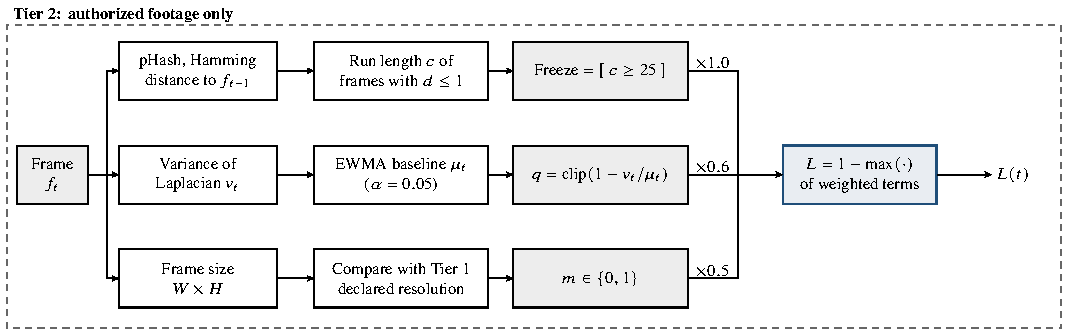
\includegraphics[width=0.92\textwidth]{fig05_tier2_liveness.pdf}
  \caption{Tier~2 frame liveness computation across perceptual-hash freeze/loop, Laplacian blur drift, and declared-resolution validation}
  \label{fig:tier2_pipeline}
\end{figure}

\subsection{Multiplicative Integrity Gate and Formal Guarantees}
Channel~B signal integrity combines both tiers via $s = (1 - \mathrm{Drift})\,L$ when Tier~2 is authorized (else $s = 1 - \mathrm{Drift}$), driving the piece-wise Integrity Gate $G(s)$ plotted in Figure~\ref{fig:gate_fn}:
\begin{equation}
  G(s) = \begin{cases}
    1, & s \ge \theta_{\mathrm{high}} = 0.85 \quad (\texttt{nominal}), \\[4pt]
    0.30 + 0.70\,\dfrac{s - 0.50}{0.85 - 0.50}, & 0.50 \le s < 0.85 \quad (\texttt{tapered}), \\[6pt]
    0.30, & s < \theta_{\mathrm{low}} = 0.50 \quad (\texttt{hard\_gated}),
  \end{cases}
  \qquad T_{\mathrm{final}} = \mathrm{round}\big(T_{\mathrm{cve}}\,G(s)\big).
\end{equation}
When $s < 0.50$, the gate enforces an explicit floor multiplier of $0.30$ and hard cap of $T_{\mathrm{final}} \le 30$. This satisfies three core properties: (i) \emph{non-compensation} (a pristine $T_{\mathrm{cve}} = 100$ camera cannot avoid \texttt{low\_trust} once $s < 0.50$), (ii) \emph{single-field tolerance} (one Tier~1 banner bump produces $\mathrm{Drift} \le 0.25$ and stays above $0.50$), and (iii) \emph{Lipschitz sensitivity} with bounded slope $2\,T_{\mathrm{cve}}$ inside the taper zone.

\begin{figure}[!ht]
  \centering
  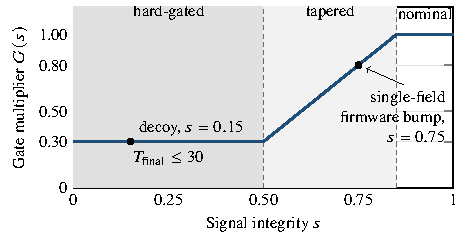
\includegraphics[width=0.72\textwidth]{fig06_gate_function.pdf}
  \caption{Multiplicative Integrity Gate $G(s)$ with thresholds $\theta_{\mathrm{low}} = 0.50$, $\theta_{\mathrm{high}} = 0.85$, floor $0.30$, and hard cap $30$}
  \label{fig:gate_fn}
\end{figure}

\section{System Design}
As illustrated in Figure~\ref{fig:arch}, COBRA-WATCH separates ingestion, scoring, and presentation across three containerized services:
\begin{itemize}
  \item \textbf{FastAPI Backend (\texttt{backend/}):} Implements REST and WebSocket endpoints (\texttt{/api/devices}, \texttt{/api/alerts}, \texttt{/api/detection-event}, \texttt{/api/ws/alerts}, \texttt{/api/censys/snapshots}, \texttt{/api/audit/*}, \texttt{/api/scenarios/run}, \texttt{/api/nl-query}) backed by SQLite with separate async/sync audit paths and $30$~s write lock timeouts. Admission controls (Figure~\ref{fig:event_pipeline}) verify constant-time \texttt{X-API-Key} authentication, 5-minute idempotency keys (HTTP~409), 10~events/min per-camera rate limits (HTTP~429), and a 60~s timestamp freshness window (HTTP~400) before persistence into the SHA-256 hash-chained \texttt{audit\_ledger}~\cite{merkle1987}. All public reads mask host octets to \texttt{/24} unless \texttt{EXPOSE\_FULL\_IP=true}.
  \item \textbf{Video AI Pipeline (\texttt{video\_pipeline/}):} Executes YOLOv8~\cite{jocher2023yolov8}, ByteTrack~\cite{zhang2022bytetrack}, spatial rule rules, and \texttt{FrameLivenessTracker} offline on whitelisted video files, pushing structured \texttt{visual\_liveness} alerts to \texttt{POST /api/detection-event}.
  \item \textbf{Next.js 16 Operator Web Application (\texttt{frontend/}):} Provides five primary routes: interactive IG-DCTF methodology overview (\texttt{/}), real-vs-synthetic research comparisons (\texttt{/research}), Gate Explorer + live WebSocket demo scenario runner (\texttt{/lab}), ethics disclosures (\texttt{/ethics}), and MapLibre GL JS triage console (\texttt{/console}) displaying self-hosted India boundaries with explicit \texttt{Simulated fixture} tags when connected to \texttt{data/public.db}.
\end{itemize}

\begin{figure}[!ht]
  \centering
  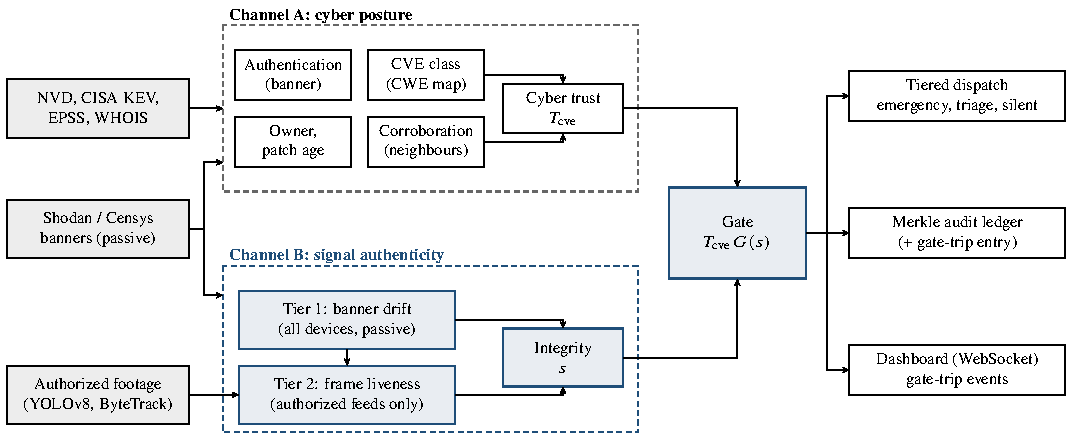
\includegraphics[width=0.95\textwidth]{fig02_architecture.pdf}
  \caption{COBRA-WATCH end-to-end passive cyber-physical architecture}
  \label{fig:arch}
\end{figure}

\begin{figure}[!ht]
  \centering
  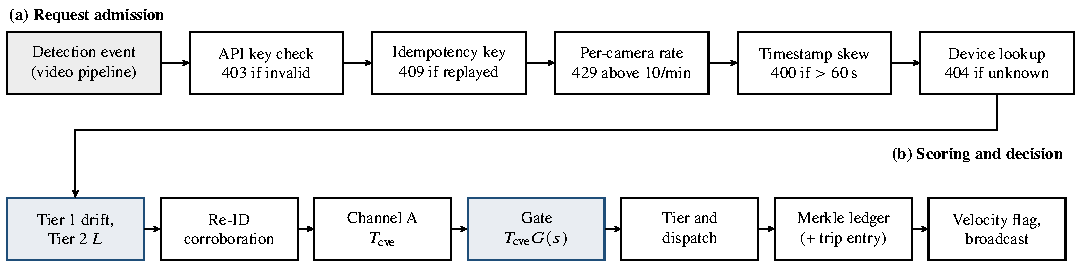
\includegraphics[width=0.95\textwidth]{fig07_event_pipeline.pdf}
  \caption{Detection event admission checks (API key, idempotency, rate limit, clock skew) prior to IG-DCTF scoring and Merkle ledger append}
  \label{fig:event_pipeline}
\end{figure}

\section{Details of Hardware and Software Requirements}
Table~\ref{tab:hw_sw} lists the verified development and evaluation stack used across Windows and Linux test hosts.

\begin{table}[!ht]
  \centering
  \caption{Hardware and software specifications}
  \label{tab:hw_sw}
  \begin{tabular}{@{}p{4.2cm}p{10.5cm}@{}}
    \toprule
    \textbf{Component} & \textbf{Specification} \\
    \midrule
    Evaluation Host & Intel Core i5-12450H CPU (CPU-only OpenCV / PyTorch inference benchmark); cross-tested on Windows~11 and Kali Linux \\
    Memory \& Storage & 16~GB RAM recommended for local Next.js~16 dev/build + YOLOv8 CPU execution; SQLite WAL storage (\texttt{public.db} $\approx 9,320$ masked rows) \\
    Backend Stack & Python 3.12.6, FastAPI, Uvicorn, Pydantic v2, aiosqlite, httpx, optional PyTorch (HTTP~503 fallback if absent) \\
    Vision \& Evaluation & OpenCV 5.0.0 / opencv-python-headless, Ultralytics YOLOv8 + ByteTrack, SciPy / Wilson \& Exact Poisson statistics \\
    Frontend Stack & Node.js ($\ge 20.9$), Next.js 16.4.0 (Turbopack), TypeScript, Tailwind CSS v4, MapLibre GL JS, Vitest 5.0.4, ESLint 9 \\
    Deployment & Docker Compose v2 (\texttt{backend}, \texttt{frontend}, \texttt{video-pipeline}) \\
    \bottomrule
  \end{tabular}
\end{table}
